\title{Relazione di ``Sistemi complessi: modelli e simulazione''}
\author{
	Simon Vocella \\
	Matricola: 718289
}
\date{\today}

\documentclass[12pt]{article}
\usepackage[margin=1.5cm]{geometry}
\usepackage[italian]{babel}
\usepackage{booktabs}
\usepackage{algorithm}% http://ctan.org/pkg/algorithm
\usepackage{algpseudocode}% http://ctan.org/pkg/algorithmicx
\usepackage{algorithmicx}
\usepackage{lipsum}% http://ctan.org/pkg/lipsum
\usepackage{float}% http://ctan.org/pkg/float
\usepackage{graphicx}
\usepackage{amsfonts}
\usepackage{amsmath}

\usepackage{listings}
\lstset{language=Java, basicstyle=\small}
\lstset{linewidth=\textwidth, showstringspaces=false}
\lstset{frame=trBL}

\begin{document}
\maketitle

\section{Il problema}
Al giorno d'oggi esistono molti sistemi di catalogazione di paper scientifici (es. DBLP). Il nostro programma si propone di fare scraping in uno o pi\`u di questi sistemi per risolvere i seguenti problemi:
\begin{itemize}
\item Calcolare un indice di similarit\`a tra i risultati raccolti nei vari siti
\item Filtrare le citazioni in Google Scholar tramite DBLP
\end{itemize}

\section{Sorgenti informative utilizzate}
In questo progetto si \`e deciso di utilizzare i seguenti sistemi di catalogazione:
\begin{itemize}
\item DBLP (http://www.informatik.uni-trier.de/$\sim$ley/db/)
\item Google scholar (http://scholar.google.it/)
\end{itemize}

\section{Approccio e metriche adottate}

\subsection{Indice di similarit\`a}
Esiste un sistema centrale che comunica ai vari agenti cosa bisogna cercare. Ogni agente \`e specializzato in un sistema di catalogazione diverso. Nel nostro caso avremo due agenti. Ogni agente far\`a scraping nel proprio sito e trasmetter\`a i risultati al sistema centrale. Man mano che ogni agente consegner\`a i propri risultati, verr\`a creata una lista $<Key, Value>$ in cui la $Key$ sar\`a il titolo del paper j-esimo e $Value$ sar\`a uguale a $\displaystyle\sum\limits_{i=0}^n i(j)/(n*m)$ dove $i(j)$ sar\`a uguale a 1, nel caso l'i-esimo agente avesse il j-esimo paper, altrimenti 0 e m e n sono rispettivamente il numero totale dei paper trovati e il numero totale degli agenti.\\
L'indice di similarit\`a sar\`a la sommatoria dei vari $Value$, $\displaystyle\sum\limits_{j=0}^m Value(j) = \displaystyle\sum\limits_{j=0}^m \displaystyle\sum\limits_{i=0}^n i(j)/(n*m)$ e in questo caso indica quanto le n liste, raccolte dagli n agenti, siano simili. \\\\
Nel caso in cui sia $\displaystyle\sum\limits_{i=0}^n i(j)/(n*m) = 1/m$ allora qualsiasi agente ha trovato il paper j-esimo.\\
Nel caso in cui l'indice di similarit\`a sia $\displaystyle\sum\limits_{j=0}^m Value(j) = \displaystyle\sum\limits_{j=0}^m \displaystyle\sum\limits_{i=0}^n i(j)/(n*m) = 1$, indica che le n liste di paper raccolte dagli n agenti sono identiche.\\

\subsection{Validazione dei paper da Google Scholar}
\`E noto che Google Scholar indicizza moltissime voci, anche non riguardanti il mondo scientifico, quindi si \`e pensato di filtrare le citazioni in Google Scholar tramite un sistema pi\`u rigoroso, DBLP, avendo cos\`i una sorta di validazione. Per ogni paper scaricato per calcolare l'indice di similarit\`a, scarichiamo $k$ citazioni, dove $k >= 0$, e ogni citazione verr\`a cercata e validata in DBLP.

\section{Architettura del sistema}
Il sistema \`e basato su un piano di controllo basato su Jason (Java-based AgentSpeak interpreter used with SACI for multi-agent distribution over the net). Il piano di controllo viene specificato tramite un file MAS (Multiple Agent System).
\lstinputlisting[caption=Il file MAS: Multiple Agent System,label=lst:java]{../bibliography.mas2j}
Il file mas2j ci permette di specificare l'architettura del nostro sistema: il tipo di infrastruttura, gli agenti che interagiscono e di quale tipo sono.
\\
\subsection{Infracstructure}
Un'infrastruttura fornisce i seguenti servizi per i MAS:
\begin{itemize}
\item comunicazione (ad esempio, le infrastrutture centralizzate implementano la comunicazione basata su KQML, mentre JADE implementa la comunicazione utilizzando FIPA-ACL)
\item il controllo del ciclo di vita dell'agente (creazione, esecuzione, distruzione)
\end{itemize}
Sono disponibili le seguenti infrastrutture:
\begin{itemize}
\item  centralizzata: \\ Questa infrastruttura esegue tutti gli agenti nello stesso host. Esso fornisce prestazioni di avvio veloci ed alte per i sistemi che possono essere eseguiti in un singolo computer. \`E  anche utile per testare e sviluppare (prototipi) sistemi. \`E l'infrastruttura di default.
\item Jade: \\ Fornisce la distribuzione e la comunicazione con Jade, che si basa su FIPA-ACL. Con questa infrastruttura, tutti gli strumenti disponibili con JADE sono disponibili anche per monitorare e controllare gli agenti Jason.
\end{itemize}
\subsection{Librarian}
L'agente principale che si occupa di prendere l'input dell'utente e cordinare il lavoro degli altri agenti \`e Librarian. Librarian \`e definito nel file asl. Grazie al fatto che nel file mas2j sia stata specificata la propriet\`a $agentArchclass$ $LibrarianGUI$, diciamo che l'architettura dell'agente \`e definita nel file LibrarianGUI.java. \\
Tramite GUI, l'utente pu\`o ricercare un qualsiasi autore dentro i siti di catalogazione e questo lancer\`a all'interno dell'agente Librarian una chiamata $search\_term$ ad ogni agente.
\lstinputlisting[caption=L'agente Librarian,label=lst:java]{../librarian.asl}
\lstinputlisting[caption=Architettura LibrarianGUI,label=lst:java]{../LibrarianGUI.java}

\subsection{DBLP e Scholar}
All'azione di $search\_term$ ogni agente comunica un azione interna di $<Agent>.scraping\_search\_term$ che comunica il termine ad un azione interna. Qui presentiamo gli agenti scholar e dblp.
\lstinputlisting[caption=L'agente Scholar,label=lst:java]{../scholar.asl}
\lstinputlisting[caption=Azione interna di scraping di Scholar,label=lst:java]{../scholar/scraping_search_term.java}
\lstinputlisting[caption=L'agente Dblp,label=lst:java]{../dblp.asl}
\lstinputlisting[caption=Azione interna di scraping Dblp,label=lst:java]{../dblp/scraping_search_term.java}
Ogni azione interna di $<Agent>.scraping\_search\_term$ comunica ad un interfaccia di scraping chiamata Session. Session, una volta istanziata, fa partire un webkit modificato che rimane in ascolto su una porta specificata o di default che chiameremo per semplicit\`a Webkit. Tramite Session comunichiamo le nostre azioni di visita al Webkit e tramite xpath manipoliamo il DOM della pagina e tramite funzioni di QT o Javascript manipoliamo funzioni come il submit, click, history, etc. \\
Ogni agente esegue il proprio scraping e raccoglie informazioni (nel nostro caso i titoli dei paper). Lo fa su una sola pagina nel caso di DBLP o su pi\`u pagine nel caso di Google Scholar.\\
Una volta avuti i risultati, l'azione interna restituisce o meglio unifica (visto che parliamo di linguaggio funzionale) il risultato. \\
Le azioni interne, in Jason, sono molto importanti, perch\`e sono le uniche che posso cambiare l'ambiente e le variabili di esecuzione. \\ 
Librarian si occuper\`a di raccogliere i paper in una HashMap e di calcolare incrementalmente l'indice di similarit\`a. 

\begin{figure}[htbp]
\centering
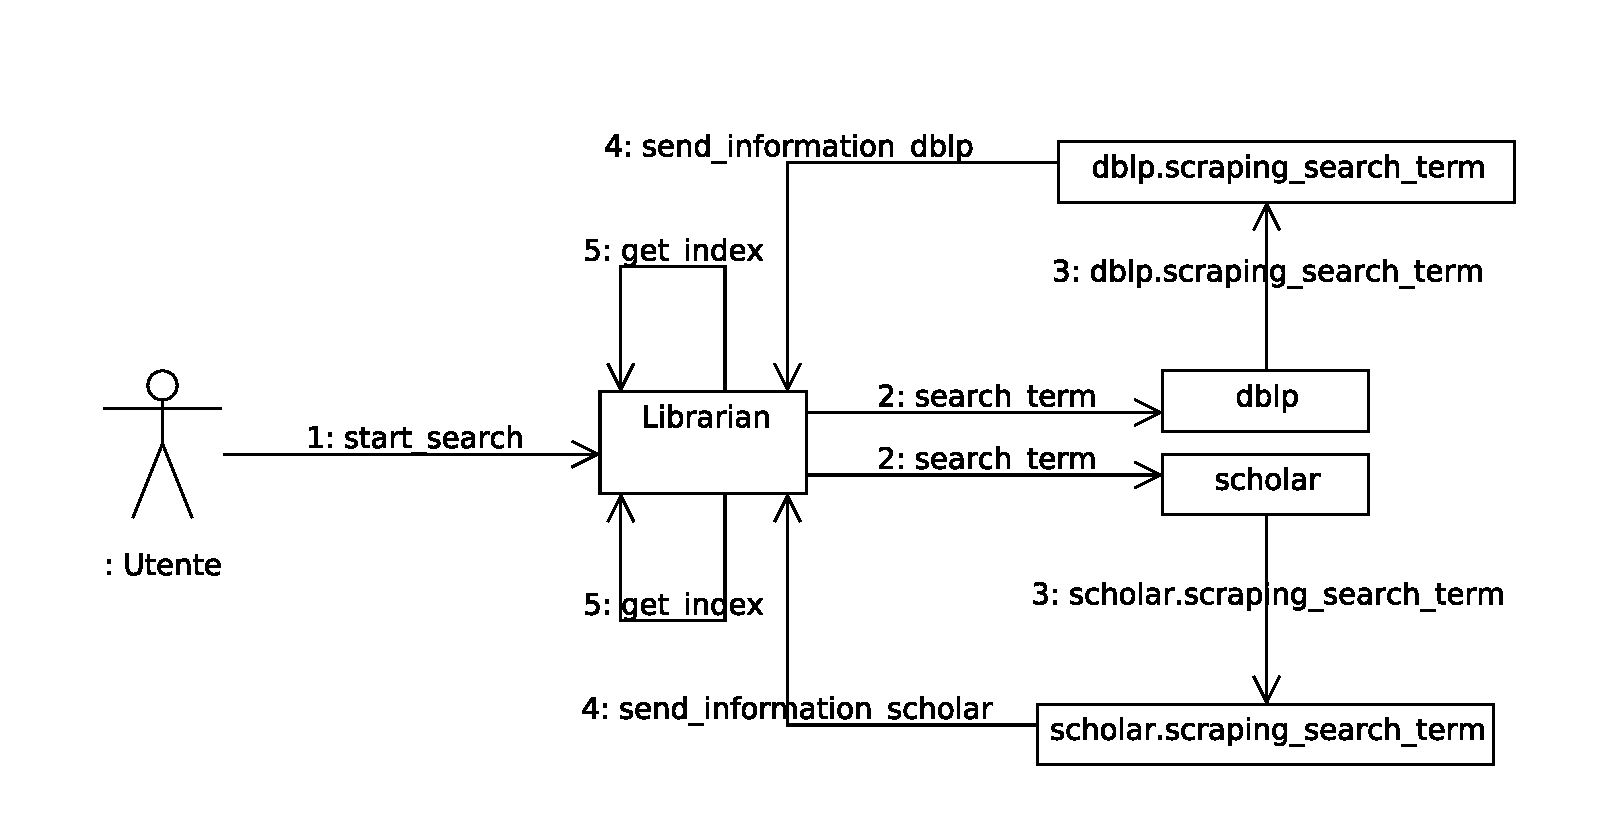
\includegraphics[width=\textwidth]{search_terms.eps}
\caption{Collaboration Diagram della ricerca}
\end{figure}

\subsection{Raccogliere e validare le citazioni}
Ora ci proponiamo di validare le citazioni raccolte in Google Scholar grazie a DBLP. L'agente Scholar, durante l'azione $scholar.scraping\_search\_term$ raccoglie anche le citazioni di ogni paper (se ne ha). Librarian si occuper\`a di rigirare la richiesta di validazione delle citazioni e contatter\`a l'agente dblp tramite l'azione $validate\_citation$, in cui si passer\`a a un azione interna $dblp.scraping\_search\_citation$ che infine resituir\`a i risultati a Librarian tramite $send\_filtered\_citations$.
\begin{figure}[htbp]
\centering
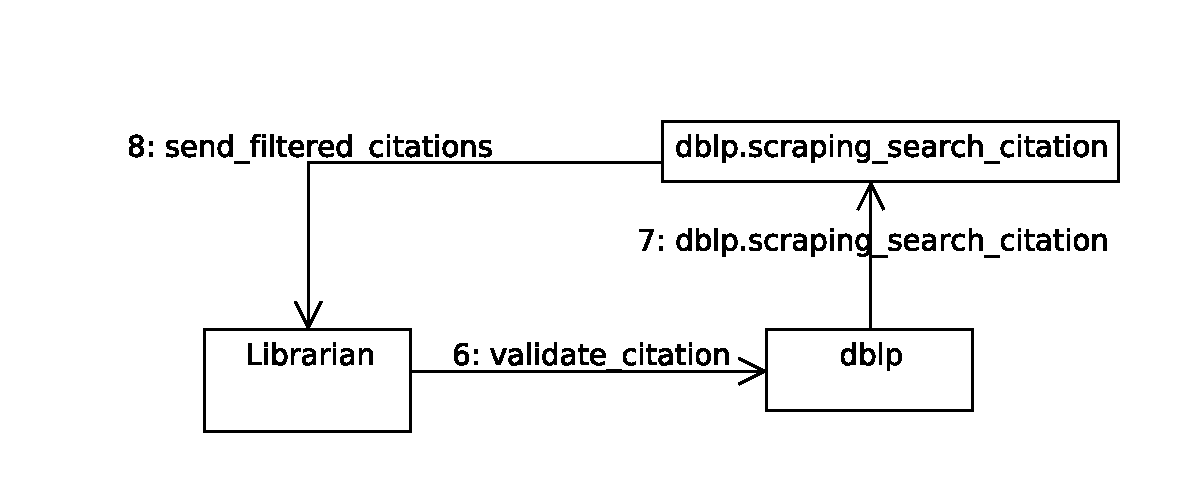
\includegraphics[width=\textwidth]{search_citation.eps}
\caption{Collaboration Diagram della validazione delle citazioni}
\end{figure}
\newpage
\lstinputlisting[caption=Azione interna di search citation di Dblp,label=lst:java]{../dblp/scraping_search_citation.java}

\section{Descrizione dei risultati}

Risultati dell'agente Dblp:
\begin{itemize}
\item An analysis of different types and effects of asynchronicity in cellular automata update schemes
\item Towards an agent-based proxemic model for pedestrian and group dynamics: motivations and first experiments
\item An Agent Model of Pedestrian and Group Dynamics: Experiments on Group Cohesion
\item An Agent-Based Proxemic Model for Pedestrian and Group Dynamics: Motivations and First Experiments
\item A Cellular Automata Based Model for Pedestrian and Group Dynamics: Motivations and First Experiments
\item ... etc.
\end{itemize}
Risultati dell'agente Scholar:
\begin{itemize}
\item Modeling dynamic environments in multi-agent simulation
\item Situated cellular agents: A model to simulate crowding dynamics
\item Situated cellular agents approach to crowd modeling and simulation
\item Awareness in collaborative ubiquitous environments: The multilayered multi-agent situated system approach
\item Toward a platform for multi-layered multi-agent situated system (MMASS)-based simulations: focusing on field diffusion
\item ... etc.
\end{itemize}
Hashmap risultante:
\begin{itemize}
\item key: Web Intelligence and Intelligent Agent Technology. Proceedings of the 2009 IEEE/WIC/ACM International Conference on Web Intelligence, Worshops, value: 0.0017857142857142857
\item key: Visualization of Discrete Crowd Dynamics in a 3D Environment, value: 0.0017857142857142857
\item key: PASSIONE STORICA E STORIA CIVICA NELLA CALABRIA NORDOCCIDENTALE. RASSEGNA BIBLIOGRAFICA E RIFLESSIONI STORIOGRAFICHE, value: 0.0017857142857142857
\item key: Le memorie del vecchio maresciallo, value: 0.0017857142857142857
\item key: Bio-ICT Convergence: Filling the Gap Between Computer Science and Biology, value: 0.0017857142857142857
\item ... etc.
\end{itemize}
Indice di similarit\`a risultante: 0.5464285714285698. \\
\\
Citazioni trovate:
\begin{itemize}
\item Agent based modeling and simulation: an informatics perspective
\begin{itemize}
	\item Modeling \& simulation of educational multi-agent systems in DEVS-suite
	\item The roundtable: an abstract model of conversation dynamics
	\item Looking at the effects of performance-based financing through a complex adaptive systems lens
	\item The Roundtable: An Agent-Based Model of Conversation Dynamics
	\item Participatory Agent-Based Simulation for Renewable Resource Management: The Role of the Cormas Simulation Platform to Nurture a Community of Practice
	\item Distributed Agent-Based Social Simulations: An architecture to simulate complex social phenomena on highly parallel computational environments
	\item Distributed Agent-Based Social Simulations: An Architecture to Simulate Complex Social Phenomena on Highly Parallel Computational Environments
	\item SimConnector: An approach to testing disaster-alerting systems using agent based simulation models
	\item IMITATIONAL MODELING OF BEHAVIOR OF LEARNING ECONOMIC AGENTS
	\item An FPGA implemented cellular automaton crowd evacuation model inspired by the electrostatic-induced potential fields
	\item Transporte colaborativo marítimo
\end{itemize}
\item Coordinated change of state for situated agents
\begin{itemize}
	\item Toward a platform for multi-layered multi-agent situated system (MMASS)-based simulations: focusing on field diffusion
	\item Dynamic interaction spaces and situated multi-agent systems: from a multi-layered model to a distributed architecture
\end{itemize}
\item Towards an agent-based proxemic model for pedestrian and group dynamic
\begin{itemize}
	\item Towards an agent-based proxemic model for pedestrian and group dynamics: motivations and first experiments
	\item Agent-based Proxemic Dynamics: Crowd and Groups Simulation
	\item Exitus: An Agent-Based Evacuation Simulation Model For Heterogeneous Populations
	\item A Cellular Automata Model for Pedestrian and Group Dynamics
	\item Agent-Based Pedestrian Modeling and Simulation
	\item Dealing with crowd crystals in MAS-based crowd simulation: a proposal
	\item An Agent-Based Approach to Pedestrian and Group Dynamics: Experimental and Real World Scenarios
\end{itemize}
\item Situated cellular agents and immune system modelling
\begin{itemize}
	\item Toward a platform for multi-layered multi-agent situated system (MMASS)-based simulations: focusing on field diffusion
	\item A model of multi-agent system based on immune evolution
	\item Supporting the application of Situated Cellular Agents in non-uniform spaces
	\item A Multi-Agent-based 3D Visualization of Stem Cell Behavior
\end{itemize}
\item A CA-Based Approach to Self-Organized Adaptive Environments: The Case of an Illumination Facility
\begin{itemize}
	\item Simulation of alternative self-organization models for an adaptive environment
	\item Modeling and programming asynchronous automata networks: The MOCA approach
\end{itemize}
\item An Asynchronous Cellular Automata-Based Adaptive Illumination Facility
\begin{itemize}
	\item A cellular automata-based modular lighting system
	\item Simulation of alternative self-organization models for an adaptive environment
	\item Self-organization models for adaptive environments: Envisioning and evaluation of alternative approaches
	\item Design and Implementation of a Framework for the Interconnection of Cellular Automata in Software and Hardware
\end{itemize}
\item etc..
\end{itemize}
Ogni citazione viene verificato se esiste o meno ricercandola in DBLP. Nel caso in cui la ricerca No hits, allora la citazione viene eliminata.

\section{Conclusioni}
Come abbiamo visto le due liste di risultati differiscono per un buon numero di paper, in questo caso \`e colpa di Scholar che mette molti altri risultati oltre agli articoli scientifici (un es. \`e PASSIONE STORICA E STORIA CIVICA NELLA CALABRIA NORDOCCIDENTALE. RASSEGNA BIBLIOGRAFICA E RIFLESSIONI STORIOGRAFICHE, value: 0.0017857142857142857, che non sembra molto avere a che fare con l'informatica). Si potrebbe migliorare il risultato, aumentando il numero di siti di catalogazione da visitare, riducendo cos\`i il peso di Scholar da 1/2 a 1/n dove n sar\`a il nuovo numero di siti scelti.\\\\
Anche nel caso della validazione delle citazioni di Google Scholar, potremmo affidarci anche ad altri siti di catalogazione e non partire dal presupposto che DBLP sia sempre infallibile.

\end{document}
